\documentclass[conference]{IEEEtran}

\usepackage{booktabs}
\usepackage{cite}
\usepackage[bottom]{footmisc}
\usepackage[utf8]{inputenc}
\usepackage{graphicx}
% epstopdf needs to be included after graphicx.
\usepackage{epstopdf}
\usepackage{listings}
\usepackage{makeidx}
\usepackage{multicol}
\usepackage{newtxtext}
\usepackage{newtxmath}
\usepackage{url}
\RequirePackage[l2tabu, orthodox]{nag}

% Allow PDF 1.7 documents to be included with \includegraphics
\pdfminorversion=7

\graphicspath{{./img/}}

% listing
\lstset{%
  language={C},
  basicstyle={\small\ttfamily},%
  identifierstyle={\small\ttfamily},%
  commentstyle={\small\itshape},%
  keywordstyle={\small\bfseries},%
  ndkeywordstyle={\small\ttfamily},%
  stringstyle={\small\ttfamily},%
  frame={tb},%
  breaklines=true,%
  columns=[l]{fullflexible},%
  numbers=left,%
  numberstyle={\scriptsize},%
  stepnumber=1,%
  numbersep=1em,%
  lineskip=-0.5ex,%
  mathescape,%
  xleftmargin=2em,%
  framexleftmargin=1.5em,%
}

\begin{document}

\title{kEDM: A Performance-portable Implementation of Empirical Dynamical Modeling}

\author{%
    \IEEEauthorblockN{%
        Keichi Takahashi, Wassapon Watanakeesuntorn, Kohei Ichikawa
    } \\
    \IEEEauthorblockA{%
        Nara Institute of Science and Technology\\
        Nara, Japan\\
        \{keichi, wassapon.watanakeesuntorn.wq0, ichikawa\}@is.naist.jp
    }
    \and
    \IEEEauthorblockN{%
        Gerald M. Pao
    } \\
    \IEEEauthorblockA{%
        Salk Institute for Biological Studies\\
        California, USA\\
        pao@salk.edu
    } \\
}

\maketitle

\begin{abstract}
    Recent rapid scale out of high performance computing systems has
    rapidly and continuously increased the scale and complexity of the
    interconnects. As a result, current static and over-provisioned
    interconnects are becoming cost-ineffective. Against this background, we have
    been working on the integration of network programmability into
    the interconnect control, based on the idea that dynamically controlling
    the packet flow in the interconnect according to the communication pattern
    of applications can increase the utilization of interconnects and improve
    application performance. Interconnect simulators come in handy especially
    when investigating the performance characteristics of interconnects with
    different topologies and parameters. However, little effort has been put
    towards the simulation of packet flow in dynamically controlled interconnects,
    while simulators for static interconnects have been extensively researched
    and developed. To facilitate analysis on the performance
    characteristics of dynamic interconnects, we have developed PFAnalyzer.
    PFAnalyzer is a toolset composed of PFSim, an interconnect simulator
    specialized for dynamic interconnects, and PFProf, a profiler.
    PFSim allows interconnect researchers and designers to investigate
    congestion in the interconnect for an arbitrary cluster configuration and
    a set of communication patterns collected by PFProf. PFAnalyzer is used
    to demonstrate how dynamically controlling the interconnects can reduce
    congestion and potentially improve the performance of applications.
\end{abstract}

\begin{IEEEkeywords}
    Simulation, Profiling, Interconnect, Message Passing Interface, Software
    Defined Networking
\end{IEEEkeywords}

\begin{figure}
    \centering
    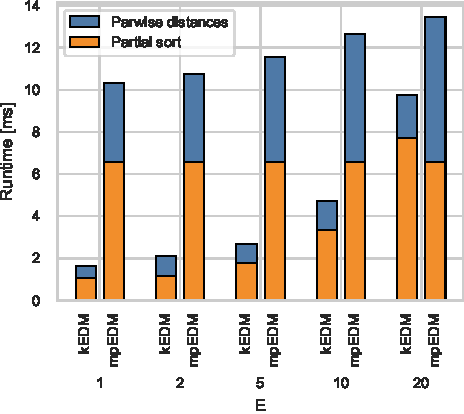
\includegraphics{figs/breakdown_v100}
    \caption{Breakdown of kNN runtime on V100}%
    \label{fig:architecture}
\end{figure}

\begin{figure}
    \centering
    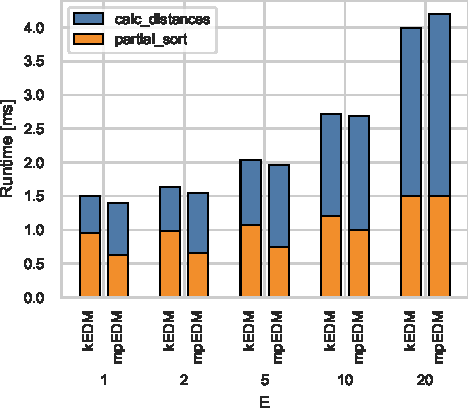
\includegraphics{figs/breakdown_epyc}
    \caption{Breakdown of kNN runtime on EPYC 7742 $\times$2}%
    \label{fig:architecture}
\end{figure}

\begin{figure}
    \centering
    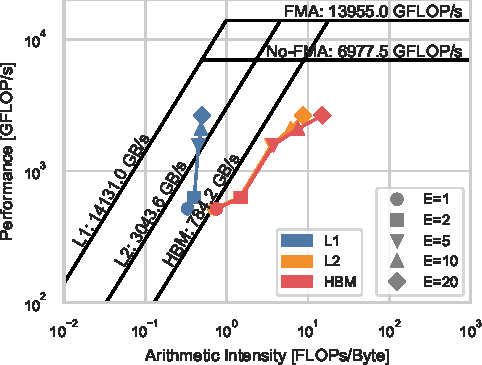
\includegraphics{figs/roofline_distances_v100}
    \caption{Roofline analysis of pairwise distance kernel on V100}%
    \label{fig:architecture}
\end{figure}

\begin{figure}
    \centering
    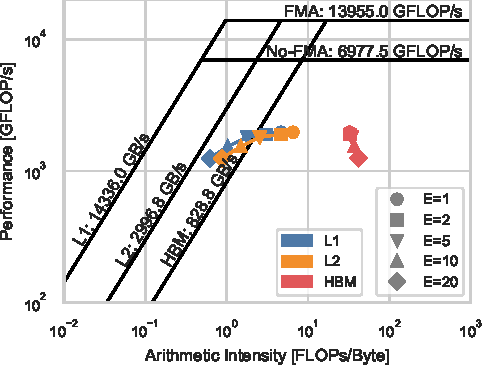
\includegraphics{figs/roofline_lookup_v100}
    \caption{Roofline analysis of lookup kernel on V100}%
    \label{fig:architecture}
\end{figure}

\begin{figure}
    \centering
    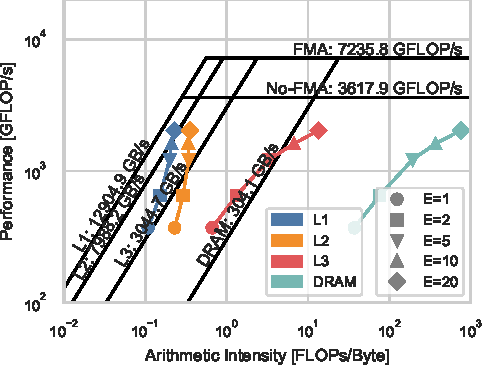
\includegraphics{figs/roofline_distances_epyc}
    \caption{Roofline analysis of pairwise distance kernel on EPYC 7742}%
    \label{fig:architecture}
\end{figure}

\begin{figure}
    \centering
    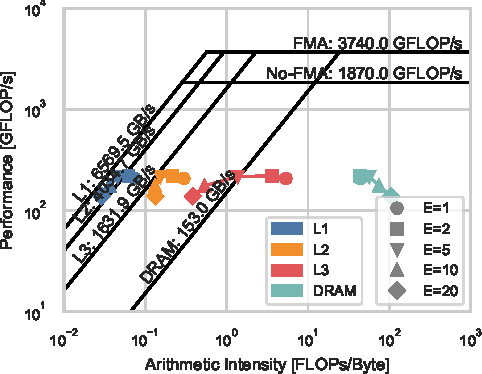
\includegraphics{figs/roofline_lookup_epyc}
    \caption{Roofline analysis of lookup kernel on EPYC 7742}%
    \label{fig:architecture}
\end{figure}



\section*{Acknowledgements}
This work was supported by JSPS KAKENHI Grant Number JP20K19808.

\end{document}
